\begin{section_3}
\subsection{Код}
\begin{lstlisting}[language=Python]
import numpy as np
import matplotlib.pyplot as plt
import os
from time import time

WIDTH = HEIGHT = 800
MAX_ITER = 10000
ESCAPE_RADIUS = 4.0

def compute_julia(c, bounds=(-1.5, 1.5), resolution=(WIDTH, HEIGHT)):
  x_min, x_max = bounds
  y_min, y_max = bounds
  cols, rows = resolution

  x = np.linspace(x_min, x_max, cols)
  y = np.linspace(y_min, y_max, rows)
  X, Y = np.meshgrid(x, y)
  Z = X + 1j * Y
  counts = np.zeros(Z.shape, dtype=np.int32)
  active = np.ones(Z.shape, dtype=bool)

  for i in range(MAX_ITER):
      Z[active] = Z[active] ** 2 + c
      mask = (Z.real**2 + Z.imag**2) > ESCAPE_RADIUS
      escaped = mask & active
      counts[escaped] = i
      active &= ~escaped
      if not np.any(active):
          break

  counts[active] = MAX_ITER
  return counts

def render_julia(image, c, output_path):
  normalized = np.log1p(image)
  normalized /= normalized.max()

  fig, ax = plt.subplots(figsize=(6, 6), facecolor='black')
  ax.imshow(normalized, extent=(-1.5, 1.5, -1.5, 1.5), cmap='magma')
  ax.axis('off')
  fig.text(0.5, 0.03, f"Параметр c = {c.real:.3f} + {c.imag:.3f}i",
           ha='center', va='center', color='white', fontsize=12)
  plt.savefig(output_path, dpi=300, bbox_inches='tight')
  plt.close(fig)

if __name__ == "__main__":
  output_dir = "tfkp"
  os.makedirs(output_dir, exist_ok=True)

  constants = [
      -0.5251993 + 0.5251993j,
      -0.70176 - 0.3842j,
      0.45 + 0.1428j,
      -0.8 + 0.156j,
      0.0 + 0.0j
  ]

  for idx, c in enumerate(constants, start=1):
      t0 = time()
      fractal = compute_julia(c)
      filename = f"julia_{idx}_{c.real:.3f}_{c.imag:.3f}.png"
      render_julia(fractal, c, os.path.join(output_dir, filename))
      print(f"Сделано {filename} за {time() - t0:.1f} cек.")

\end{lstlisting}
\subsection{Картинки}
\begin{figure}
    \centering
    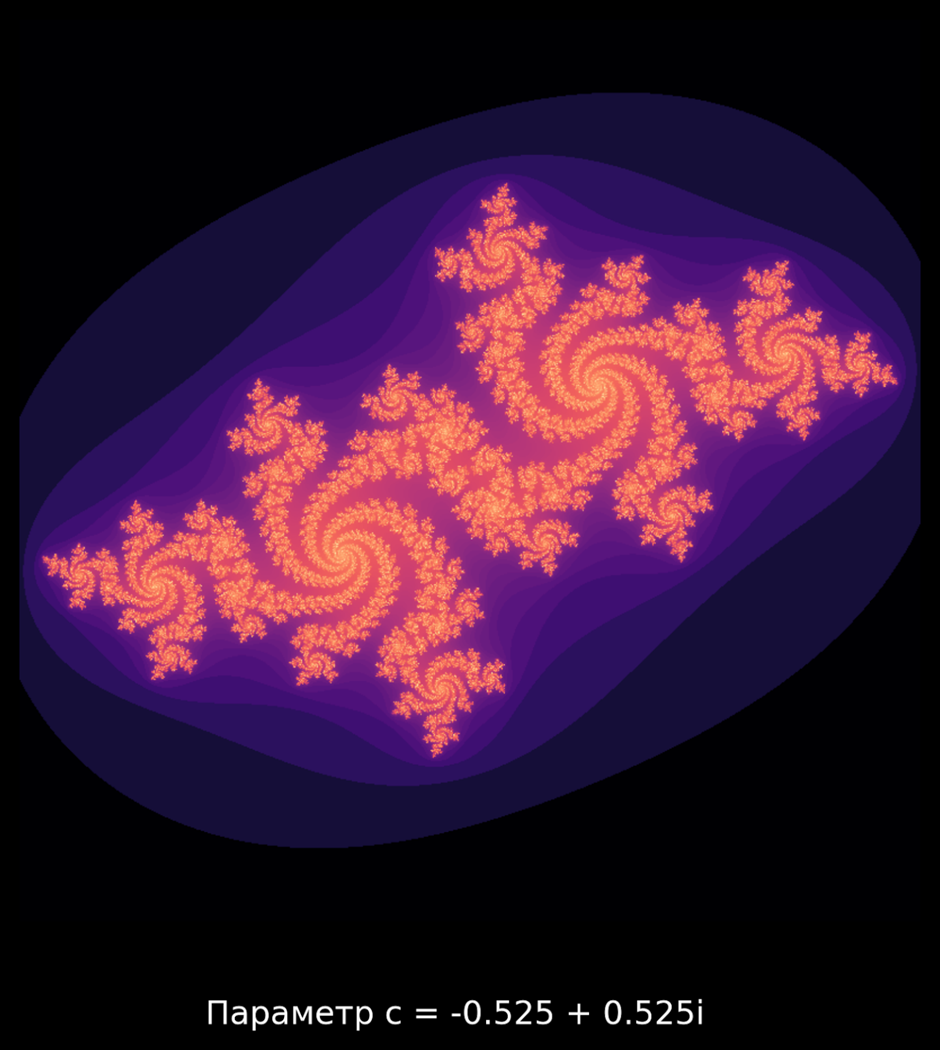
\includegraphics[width=1\linewidth]{photo/image6.png}
    \label{fig:placeholder}
\end{figure}
\begin{figure}
    \centering
    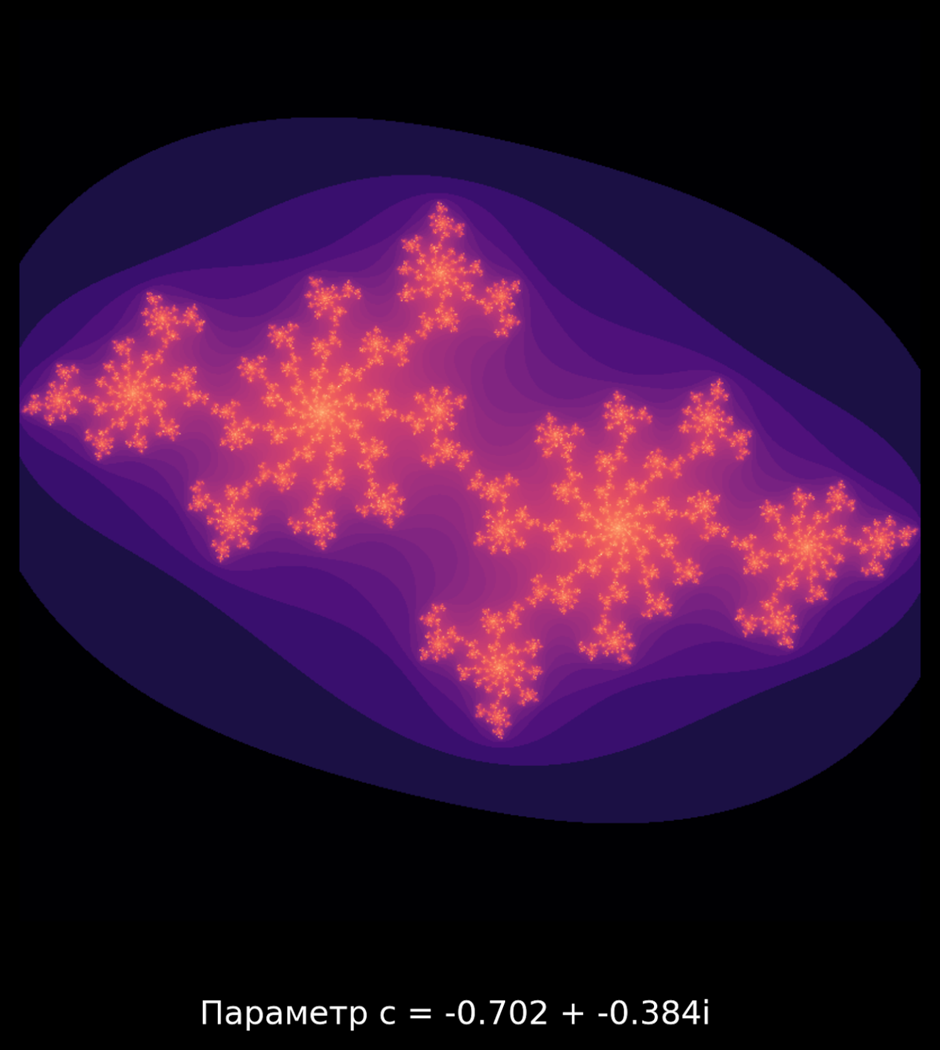
\includegraphics[width=1\linewidth]{photo/image7.png}
    \label{fig:placeholder}
\end{figure}
\begin{figure}
    \centering
    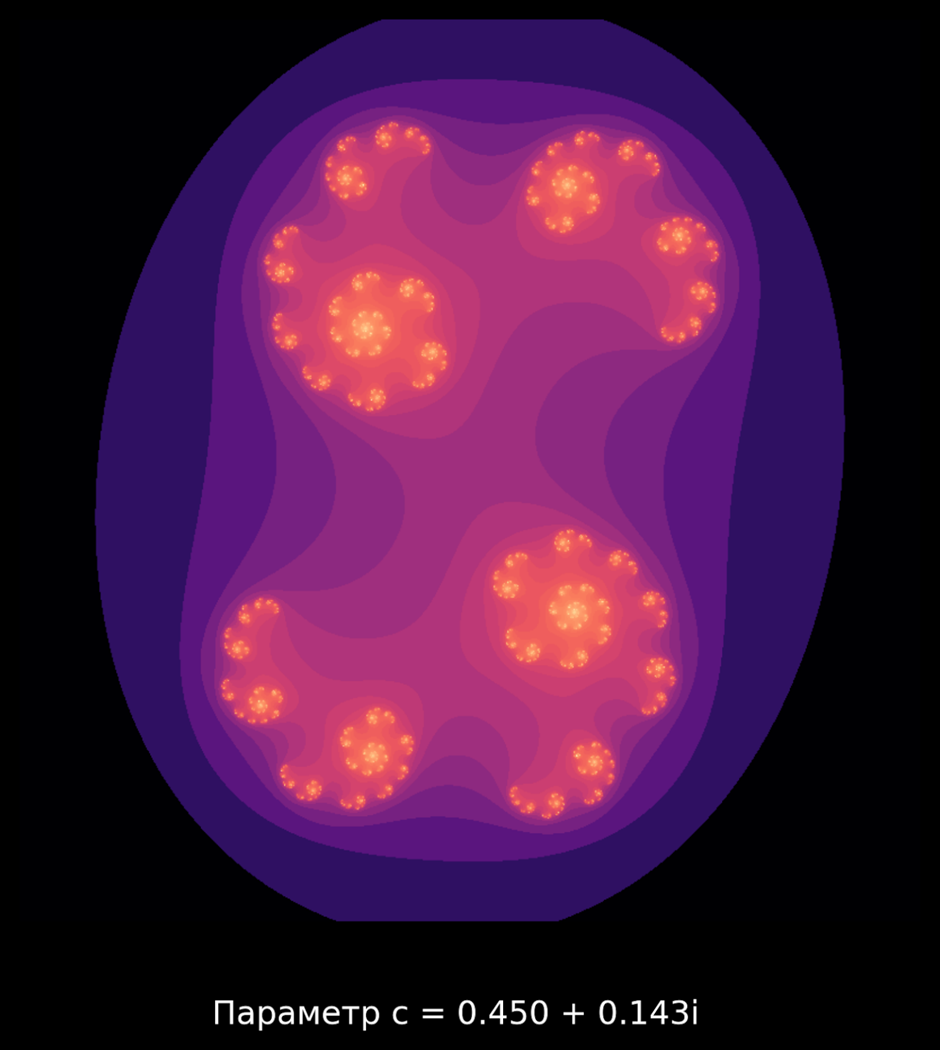
\includegraphics[width=1\linewidth]{photo/image8.png}
    \label{fig:placeholder}
\end{figure}
\begin{figure}
    \centering
    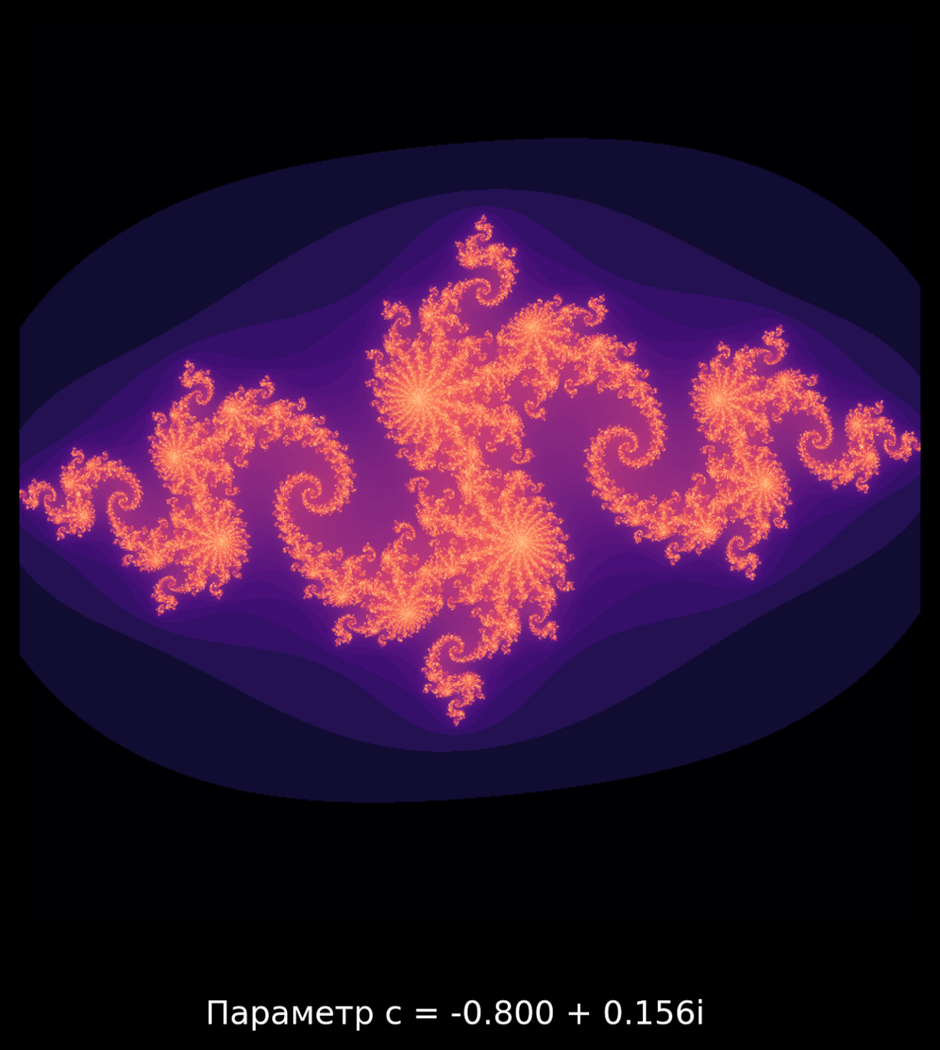
\includegraphics[width=1\linewidth]{photo/image9.png}
    \label{fig:placeholder}
\end{figure}
\begin{figure}
    \centering
    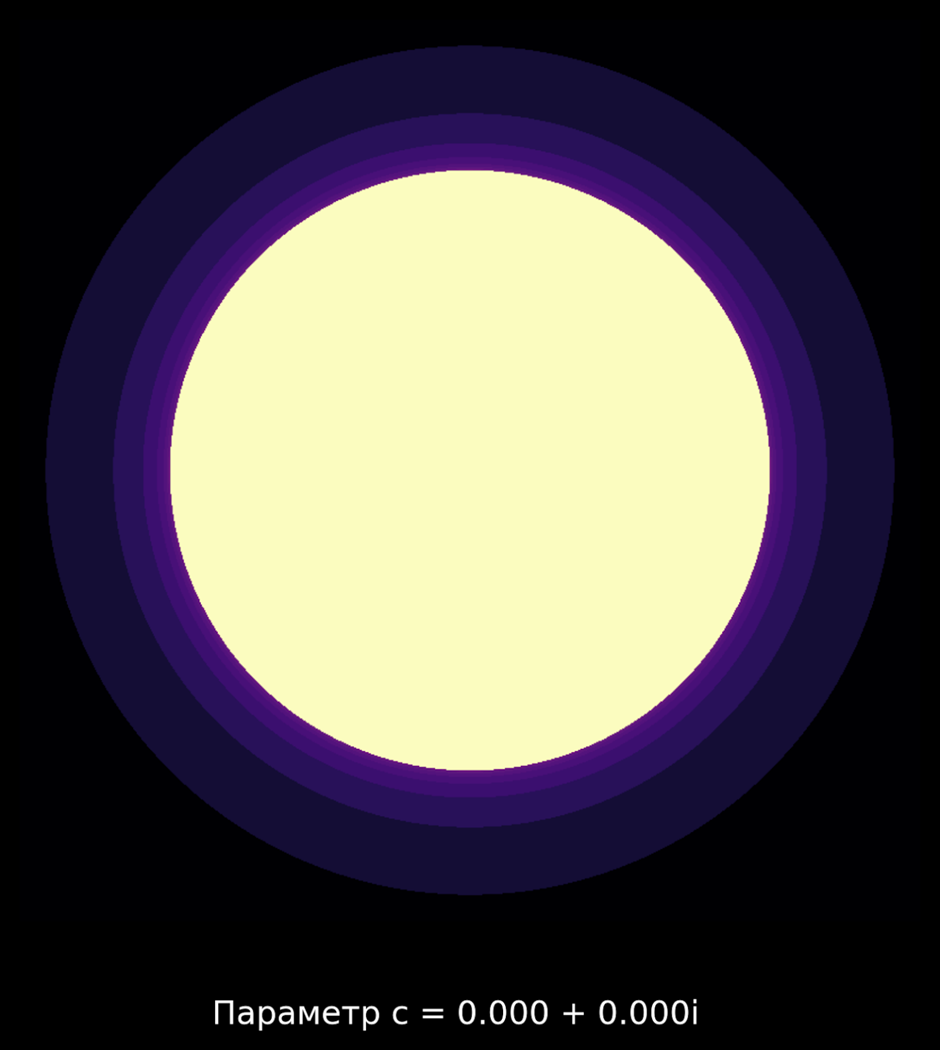
\includegraphics[width=1\linewidth]{photo/image10.png}
    \label{fig:placeholder}
\end{figure}
\end{section_3}